\documentclass[a4paper,12pt]{report}

% Encodage et langue
\usepackage[utf8]{inputenc}
\usepackage[T1]{fontenc}
\usepackage[french]{babel}

% Mise en page
\usepackage{geometry}
\geometry{margin=2.5cm}

% Packages utiles
\usepackage{graphicx}  % Pour les images
\graphicspath{{images/}}

\usepackage{amsmath, amssymb}  % Pour les maths
\usepackage[hidelinks]{hyperref}  % Pour les liens
\usepackage{float}  % Pour le placement des figures

\title{ Introduction au Data Mining}
\author{DNJOMOU YONMBA WILFRIED LOIC CM-UDS-24SCI0999 \\
KENFACK LEONEL CM-UDS-17SCI0998\\
SAGUEU WAKAM DILANE CM-UDS-24SCI1040\\}
\date{Mars 2024}

\begin{document}

\maketitle

\tableofcontents

\chapter*{Introduction Générale}
Présentation générale du sujet et des objectifs du rapport.

\chapter{Définition et Enjeux du Data Mining}
Présentation du sujet et des objectifs du rapport.

\section{Méthodologie}
Description des méthodes utilisées.

\chapter{Mise en oeuvre d’un projet de DM}
Présentation du sujet et des objectifs du rapport.

\section{Le processus de découverte de connaissances (kdd)}
Face à l'énorme quantité de données stockées dans des fichiers, des bases de données et autres référentiels, il est de plus en plus important, voire nécessaire, de développer des outils performants d'analyse et d'interprétation de ces données, ainsi que d'extraction de connaissances pertinentes susceptibles d'aider à la prise de décision.
L'exploration de données, également appelée découverte de connaissances dans les bases de données (KDD: Knowledge Discovery in Databases), désigne l'extraction non triviale d'informations implicites, jusqu'alors inconnues et potentiellement utiles, à partir de données stockées dans des bases de données. Bien que le data mining et la découverte de connaissances dans les bases de données (KDD) soient souvent considérées comme des synonymes, le data mining fait en réalité partie du processus de découverte de connaissances. La figure suivante (Figure 2.1) illustre l'exploration de données comme une étape d'un processus itératif de découverte de connaissances.

\begin{figure}[h]
    \centering
    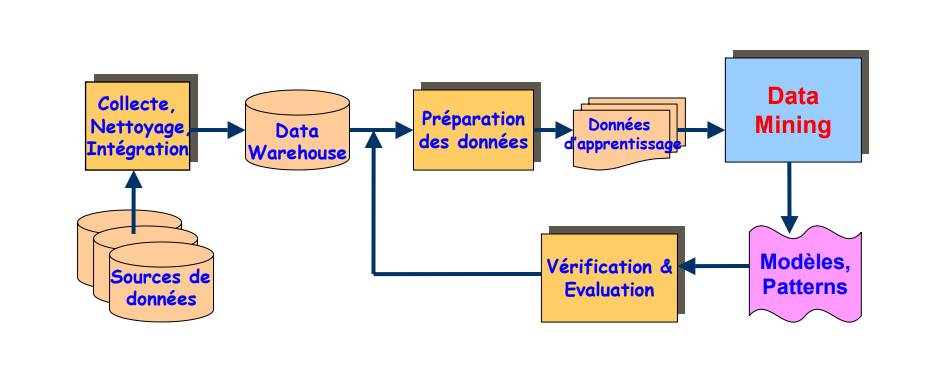
\includegraphics[width=0.75\textwidth]{KDD$data_mining}
    \caption{Data mining : coeur de KDD.}
    \label{fig:mesh1}
\end{figure}

Le processus de découverte de connaissances dans les bases de données comprend plusieurs étapes, allant de la collecte de données brutes à la production de nouvelles connaissances. Ce processus itératif comprend les étapes suivantes.

\begin{itemize}
  \item \textbf{Nettoyage des données} : il s’agit d’une phase au cours de laquelle les données parasites et les données non pertinentes sont supprimées de la collection.
  \item \textbf{Intégration des données} : à ce stade, plusieurs sources de données, souvent hétérogènes, peuvent être combinées en une source commune.
  \item \textbf{Sélection des données} : à cette étape, les données pertinentes pour l’analyse sont sélectionnées et extraites de la collecte de données.
  \item \textbf{Transformation des données} : également appelée consolidation des données, il s’agit d’une phase au cours de laquelle les données sélectionnées sont transformées sous des formes adaptées à la procédure d’exploration.
  \item \textbf{Exploration des données} : étape cruciale où des techniques astucieuses sont appliquées pour extraire des modèles potentiellement utiles.
  \item \textbf{Évaluation des modèles} : à cette étape, des modèles strictement intéressants représentant les connaissances sont identifiés sur la base de mesures données.
  \item \textbf{Représentation des connaissances} : phase finale au cours de laquelle les connaissances découvertes sont représentées visuellement à l’utilisateur. Cette étape essentielle utilise des techniques de visualisation pour aider les utilisateurs à comprendre et à interpréter les résultats de l’exploration des données. \\
  
\end{itemize}

Il est courant de combiner certaines de ces étapes. Par exemple, le nettoyage et l'intégration des données peuvent être réalisés conjointement lors d'une phase de prétraitement afin de générer un entrepôt de données. La sélection et la transformation des données peuvent également être combinées lorsque la consolidation des données résulte de la sélection ou, comme dans le cas des entrepôts de données, lorsque la sélection est effectuée sur des données transformées.

Le KDD est un processus itératif. Une fois les connaissances découvertes présentées à l'utilisateur, les mesures d'évaluation peuvent être améliorées, l'exploration peut être affinée, de nouvelles données peuvent être sélectionnées ou transformées, ou de nouvelles sources de données peuvent être intégrées, afin d'obtenir des résultats différents et plus pertinents.

Le data mining tire son nom des similitudes entre la recherche d'informations précieuses dans une grande base de données et l'extraction de minerais précieux. Ces deux techniques impliquent soit de passer au crible une grande quantité de matériaux, soit de sonder ingénieusement ces matériaux pour identifier précisément où se trouvent les valeurs. Il s'agit toutefois d'une appellation erronée, car l'extraction de l'or dans les roches est généralement appelée « extraction d'or » et non « extraction de roches ». Par analogie, l'exploration de données aurait donc dû être appelée « exploration de connaissances ». Néanmoins, l'exploration de données est devenue le terme courant et, très rapidement, une tendance qui a même éclipsé des termes plus généraux tels que la découverte de connaissances dans les bases de données (KDD), qui décrit un processus plus complet. D'autres termes similaires font référence à l'exploration de données : dragage de données, extraction de connaissances et découverte de modèles.

\section{Démarche méthodologique du Data Mining}
     \subsection{Comprendre l’application}
         Avant d’exploiter les données, il est crucial de bien comprendre le contexte d’application. Cette phase initiale permet d’identifier les objectifs du projet, les connaissances préalables disponibles et les attentes des utilisateurs finaux. Il s’agit de répondre à plusieurs questions essentielles : quel problème cherche-t-on à résoudre ? Quels sont les bénéfices attendus ? Quelles sont les contraintes à prendre en compte ? Une bonne compréhension du domaine d’étude oriente les choix méthodologiques et facilite l’interprétation des résultats obtenus.

     \subsection{Sélectionner un échantillon de données}
         Une base de données peut contenir des millions d’enregistrements, mais il est souvent inefficace, voire impossible, d’analyser l’ensemble des données en une seule fois. Il est donc nécessaire de sélectionner un échantillon représentatif. Cette étape implique le choix d’une méthode d’échantillonnage adaptée :
    
         \begin{itemize}
             \item \textbf{Échantillonnage aléatoire} : sélection d’un sous-ensemble de données de manière aléatoire.
        
             \item \textbf{Échantillonnage stratifié} : division des données en groupes homogènes avant la sélection.
        
             \item \textbf{Échantillonnage basé sur des critères spécifiques} : choix d’un échantillon répondant à certaines conditions précises.
         \end{itemize}
    
        Un échantillonnage pertinent garantit une bonne représentativité et permet d’effectuer des analyses plus rapides et précises.

     \subsection{Nettoyage et transformation des données}

         Les données brutes sont souvent imparfaites : elles peuvent contenir des valeurs manquantes, des incohérences ou des erreurs de saisie. Il est donc impératif de nettoyer et de transformer les données avant de les exploiter. Cette phase inclut :
         \begin{itemize}
             \item \textbf{Suppression du bruit} : élimination des données superflues, marginales ou erronées.
    
            \item \textbf{Gestion des valeurs manquantes} : suppression, estimation ou imputation des valeurs absentes.
    
             \item \textbf{Réduction de la dimensionnalité} : sélection des attributs les plus pertinents pour diminuer la complexité du problème.
         \end{itemize}
         
    
         Un bon prétraitement des données améliore la qualité des modèles et évite d’obtenir des résultats biaisés.

     \subsection{Appliquer les techniques de fouille de données}

         Une fois les données préparées, les techniques de Data Mining peuvent être appliquées. Le choix des algorithmes dépend du type de problème à résoudre :
    
         \begin{itemize}
             \item \textbf{Classification} : attribution d’une catégorie à chaque observation (ex. : arbres de décision, réseaux de neurones, SVM).
        
             \item \textbf{Clustering} : regroupement des données en classes homogènes sans étiquette prédéfinie (ex. : k-means, DBSCAN).
        
             \item \textbf{Règles d’association} : détection de relations entre les attributs des données (ex. : algorithmes Apriori, FP-Growth).
        
             \item \textbf{Détection d’anomalies} : identification de valeurs atypiques dans un ensemble de données (ex. : isolation forest, SVM à une classe).
         \end{itemize}
    
         Le choix du bon algorithme dépend de la nature des données et des objectifs fixés.

     \subsection{Visualiser, évaluer et interpréter les modèles}
         Après l’application des algorithmes, il est essentiel d’évaluer la qualité des modèles obtenus. Cette phase comprend :
    
         \begin{itemize}
             \item \textbf{Analyse de la pertinence des résultats} : mesure de la valeur ajoutée par les connaissances découvertes.
        
             \item \textbf{Vérification de la validité} : test des modèles sur un jeu de données indépendant pour éviter le surapprentissage.
        
             \item \textbf{Amélioration continue} : ajustement des paramètres, sélection d’autres algorithmes si les résultats ne sont pas satisfaisants.
         \end{itemize}
    
         L’évaluation rigoureuse permet de garantir que les modèles sont exploitables et fiables.    

     \subsection{ Gérer et exploiter la connaissance découverte}
         Une fois les modèles validés, les connaissances extraites doivent être mises à disposition des décideurs ou intégrées dans des systèmes d’aide à la décision. Cela peut se faire sous différentes formes :

         \begin{itemize}
             \item \textbf{Tableaux de bord et rapports} : visualisation des résultats pour une prise de décision éclairée.
        
             \item \textbf{Intégration avec d’autres systèmes} : utilisation des résultats dans des bases de données, des systèmes experts ou des plateformes d’IA.
        
             \item \textbf{Partage et échange des connaissances} : mise en réseau des découvertes avec d’autres applications ou services.
         \end{itemize}
         Cette dernière étape assure que le travail réalisé en Data Mining a un impact concret et opérationnel.
     

\chapter{ Principales Techniques du Data Mining}
Présentation du sujet et des objectifs du rapport.

\section{Exploration et prétraitement des données }

\section{Types d’apprentissage }



\chapter{Outils et Langages utilisés}
Présentation du sujet et des objectifs du rapport.

\section{Méthodologie}
Description des méthodes utilisées.

\chapter{Défis et Limites du Data Mining}
Présentation du sujet et des objectifs du rapport.

\section{Méthodologie}
Description des méthodes utilisées.



\bibliographystyle{plain} % Style de la bibliographie
\bibliography{references} % Fichier BibTeX (references.bib)

\end{document}
